\newsection{Intermediate}

\underline{\textlg{\textbf{Questions are continued on the next page}}}
\newpage
\begin{enumerate}
  
\item \textbf{Given a string, swap the vowels on opposite sides of the string.}
\begin{consolethree}
Example:
Input: "IceCreAm"
Output: "AceCreIm"
\end{consolethree}
\newpage



\item \textbf{You are given a positive integer n that specifies the size of an n x n matrix.}

Your goal is to construct a matrix of that size where the elements are ordered in spiral order between 1 and $n^2$ (image below)


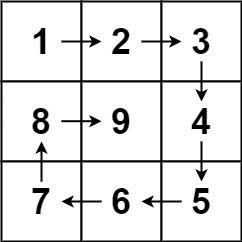
\includegraphics[scale=0.45]{images/spiral-mtx.jpg}


\begin{consolethree}
Example 1:
Input: 3
Output: [[1,2,3],[8,9,4],[7,6,5]]

Example 2:
Input: 2
Output: [[1,2],[4,3]]

Example 3:
Input: 1
Output: [[1]]
\end{consolethree}
\newpage


\item \textbf{Given the coordinates of the corners for 2 rectangles, find the area of the 2 rectangles.}

  
  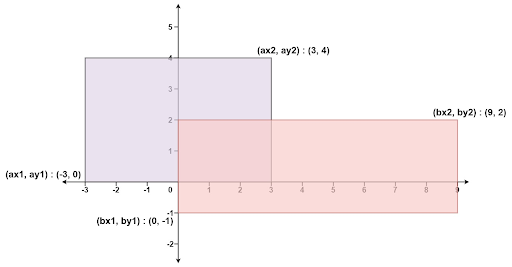
\includegraphics[scale=0.45]{images/coords.png}

  
\begin{consolethree}
Example 1: -3, 0, 3, 4, 0, -1, 9, 2
Output:    45

Explanation:
6*4 = 24 and 9*3 = 27 would be 51, but they overlap.

The overlapping area is 3*2=6, so the total area of the rectangles is 45.
\end{consolethree}
\newpage


\item \textbf{Given an array of integers in the range \texttt{[0,n]}, find the missing number in that range.}
\begin{consolethree}
Example 1: [3,0,1]
Output:    2

Example 2: [9,6,4,2,3,5,7,0,1]
Output:    8

\end{consolethree}
\newpage


\item \textbf{Given an integer n, return the count of prime numbers less than n.}

\begin{consolethree}
Example: 10
Output:  4
Explanation: 2, 3, 5, 7
\end{consolethree}
\newpage


\item \textbf{Given a string representing an Excel column title, find the corresponding column number.}

\begin{consolethree}
Example 1: "A"
Output:    1

Example 2: "AA"
Output:    27

Example 3: "ZY"
Output:    701
\end{consolethree}
\newpage


\item \textbf{Given an integer, convert it to a string representing an Excel column title.}

\begin{consolethree}
Example 1: 5
Output:    "E"

Example 2: 27
Output:    "AA"

Example 3: 701
Output:    "ZY"
\end{consolethree}
\newpage


%% \item \textbf{Given a sorted array of non overlapping intervals (an array representing the start and end values of an interval) and another interval newInterval, insert newInterval so the array of intervals is still sorted and non overlapping.}

%% \emph{(This may involve merging newInterval with existing intervals.)}

%% \begin{consolethree}
%% Example 1:  [ [1, 3], [6, 9] ],
%% 			  	  newInterval = [2, 5]
%% Output:     [ [1, 5], [6, 9] ]

%% Example 2:  [ [1,2], [3,5], [6,7], [8,10], [12,16] ],
%% 			      newInterval = [4,8]
%% Output:     [ [1,2], [3,10], [12,16] ]
%% \end{consolethree}
%\newpage


\item \textbf{Given an array of integers representing the maximum number of indexes you can move, check if you can reach the end of the array.}

You start at index 0, you want to reach the end, you can move UP TO n spaces from your current position where n is the value at arr[index]; return true or false depending on if you can or cannot reach the end

\begin{consolethree}
Example 1: [2, 3, 1, 1, 4]
Output:    true

Example 2: [3, 2, 1, 0, 4]
Output:    false
\end{consolethree}
\newpage


\item \textbf{You are given an array of intervals, each element of this array is another array with length 2 that specified the start and end of the interval as follows: [start, end]. Your goal is to merge any overlapping intervals.}

\begin{consolethree}
Example 1: [[1,2],[2,3],[3,5],[8,18]]
Output:    [[1,3],[3,5],[8,18]]

Explanation: Since intervals [1,2] and [2,3] overlap, merge them into [1,3].

Example 2: [[1,5],[4,9]]
Output:    [[1,9]]

Explanation: Intervals [1,5] and [4,9] are considered overlapping.

Example 3: [[0, 10],[1,2], [3,4], [4,5]]
Output:    [[0, 10]]

Explanation: All intervals overlap with [0,10]
\end{consolethree}
\newpage


\item \textbf{Given a string consisting of words separated by spaces, modify that string according to Goat Latin rules.}          
\begin{itemize}
\item If a word starts with a vowel, add "ma" to the end of that word\\
  ``\texttt{apple}'' becomes ``\texttt{applema}''
\item If a word starts with a consonant, move the first letter to the end of the word and add ``ma''\\
  ``\texttt{goat}'' becomes ``\texttt{oatgma}''
\item Add n ``a'''s to the end of each word, where n is the word's index + 1
\end{itemize}

\begin{consolethree}
  Example: "goats eat apples"
  Output: "oatsgmaa eatmaaa applesmaaaa"
\end{consolethree}
\newpage


\end{enumerate}
